\section{Physical view}
In de physical view wordt er gekeken naar hoe het systeem gedeployed moet worden en waar.
Om dit in beeld te brengen is er gebruikgemaakt van een development diagram.
In figuur \ref{fig:DeploymentDiagram} is te zien dat er gebruik gemaakt van Docker.
Docker is een middel waarmee je software kan laten draaien op elke machine \Parencite{Docker}.
Er is voor gekozen om docker te gebruiken, zodat Snakeware niet aan een cloud provider vast hoeft te zitten.

\whitespace
\begin{graphic}
    \captionsetup{type=figure}
    \caption{Deployment diagram van het afstudeer product}
    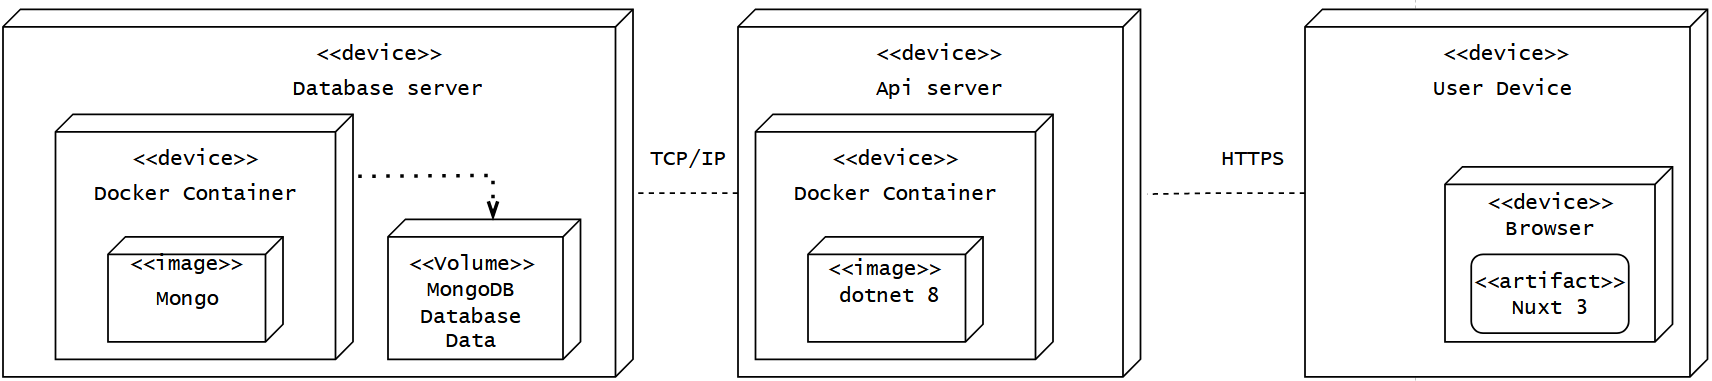
\includegraphics[scale=0.3]{DeploymentDiagram.png}
    \label{fig:DeploymentDiagram}
\end{graphic}
